\subsection{Datenbankdesign}

Das Konzept des Datenbankdesigns wird bereits unter Punkt "'Lösungswege"' behandelt.

Hinzu kommt noch das das Monitorsystem.

\subsubsection{Monitorsystem}

Damit die Monitore einen Supplierplan anzeigen können, müssen jeder Monitor einer Abteilung zugeordnet sein.\\
Auch müssen die Monitore damit sie die Raumstundenpläne anzeigen können, mit einem Raum verknüpft sein.\\
\\
Zusätzlich dazu sollen die Monitore wissen, was sie anzeigen sollen (Stundenplan, Supplierplan, Bilder, etc). Hierzu wird eine Tabelle für den Typ des Monitors erstellt und diese verknüpft.\\
\\ 
Für die Erweiterung des Monitorsystem um das Display-Steuer-System muss eine weitere Tabelle für die Display-Typ (permanent ein, permanent aus, automatisch) vorgesehen und verknüpft werden (für Details, siehe Bericht "'Display-Steuerung"' am Anhang).\\
\\
Es ergibt sich folgendes Datenbank-Layout für die Monitore:
\begin{figure}[H]
\centering
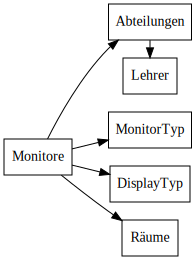
\includegraphics[keepaspectratio=true, width=7cm]{images/dbMonitors.png}
\caption{Supplierungs-Datenbank}
\end{figure}
